\section{Abstract}
In this computer based test we are asked to perform Bayesian classification on a given data set. The classification methods used are the following:
\begin{itemize}
	\item Maximum Likelihood (ML)
	\item Maximum Likelihood without Naive assumption (MLWON)
	\item Maximum A Posteriori (MAP)
	\item Maximum A Posteriori without Naive assumption(MAPWON)
\end{itemize}

We are given a data set of healthy and diseased patients to train the 4 classifiers on. Once trained, we use the classifiers to assess 2000 unclassified data and label each patient (data point / example) as diseased or healthy.

We are also asked to compare and discuss the results of the different methods. In short...

- ML showed general trend of increase in concentration, increased likelihood of diseased patient. If both chemicals went to extreme values, would likely become healthy again. Flaw in ML
- MLWON showed similar trend but was thinner and showed a downward trend due to the dependence between attributes. Definitely showed healthy patients again, unlikely.

ML and MAP were very similar. Difference of only 62 and 15 for Naive and without Naive, respectively. Likely because prior has no affect on this amount of data.

The analysis was performed in Matlab, and the code listings can be found in Appendices A, B, C, and D.

\section{Scope}
The report consists of the following structure.

\begin{enumerate}
	\item Overall Task
		\subitem Details of task set out in the ``Computer Based Test 2.''
	\item Maximum Likelihood (ML)
		\subitem Discussion on training the ML with and without the Naive assumption
		\subitem Interpretation of results
	\item Maximum A Posteriori (MAP)
			\subitem Discussion on training the MAP with and without the Naive assumption
			\subitem Interpretation of results
	\item Maximum Likelihood VS Maximum A Posteriori
			\subitem Difference of ML and MAP
			\subitem Affects of Difference on this data 
\end{enumerate}

\section{Overall Task}
We are asked to determine if a patient is diseased or healthy from a given data set. A new test is in development and measures the concentration of 2 chemicals in urine samples. 500 patients provide urine samples and also undergo a blood tests to classify if they are diseased or healthy. Thus, we have a 500 by 2 data set which is plotted in Figure \ref{fig:trainingData}. 

\begin{figure}[h]
	\centering
	\includegraphics[width=0.8\linewidth]{images/MLtrainingData}
	\caption{Training Data for the 4 methods outlined in this report. Note the imbalanced amount of healthy to diseased patients.}
	\label{fig:trainingData}
\end{figure}

We use this data set to train the 4 following methods.

\begin{itemize}
	\item Maximum Likelihood (ML)
	\item Maximum Likelihood without Naive assumption (MLWON)
	\item Maximum A Posteriori (MAP)
	\item Maximum A Posteriori without Naive assumption(MAPWON)
\end{itemize}

Once trained, we are tasked with classifying 2000 new urine samples. We use the 4 methods outlined previously to determine whether a `patient' is diseased or healthy.

It is helpful to state a hypothesis for assessment. Considering the data in Figure \ref{fig:trainingData} the hypothesis is, an increase in concentration of chemical 1 and 2 increases the likelihood of a patient being diagnosed as diseased.

%When training the Bayesian classifier we assume a Gaussian distribution as it is a ``real world'' data set, meaning it is random due to many influences and errors (e.g. input, testing errors). We expect the class-attribute to be centred evenly around some mean. The central limit theorem (CLT) reinforces this assumption by stating the shape of the distribution approaches normal as the sample size increases.



\section{Maximum Likelihood (ML)}{\label{s1}
	
\subsection{Introduction}\label{Int}
In Task 1, we are asked to ``train the Bayesian classifier, with maximum likelihood estimate (ML), on the training data with and without the Naive assumption.'' The data set is the one shown in \ref{fig:trainingData}. Once trained we classify 2000 new data points (patients).

To train ML with the Naive assumption first compute the mean and variance of the data for each class and attribute. As it is Naive, we assume the attributes (chemical 1 and 2) are independent. Armed with the mean, variance, and the new data set we use the Gaussian expression to compute the likelihood of each data point as either diseased or healthy. In this case, we are looking at the maximum likelihood and thus, only use class-conditional likelihood to classify. 

To train ML without the Naive assumption is similar to before. We compute the mean as normal but this method requires the covariance not variance of the classes and attributes. This assumes a dependence between the attributes which is useful to look at if there are not many attributes. We then compute the maximum likelihood as normal but accounting for the 3 dimensional matrix due to the covariance.

\subsection{Results}\label{CVcons}
 Figure \ref{fig:ML} shows the likelihood of being diseased or healthy depending on the concentration of the 2 chemicals. It shows there is some relationship with the concentration of the 2 chemicals and if a patient is healthy or diseased.  It shows that an increase in chemical concentration insreases likelihood of being diseased to a point. After which the likelihood starts decreasing. This seems like a flaw in the classifier or an error in the measurements but we cannot be certain. To clarify this issue we require further testing over a greater range of chemical concentration.
 
 If the data were to extend further with high concentration in both directions, we would likely see an ellipse or sphere of diseased patients. This spherical shape is due to the naive assumption which means the attributes (concentrations) are independent of each other.
 
 The trend of this data is investigated further in following sections via density and probability contour plots.
 
% It is indicated that an increase in chemical 1 concentration increases likelihood of being diseased but the level of chemical 2 concentration has varying results. There is a maximum of its 
\begin{figure}[h]
	\centering
	\includegraphics[width=0.8\linewidth]{images/MLnewData}
	\caption{Maximum Likelihood classification of new data}
	\label{fig:ML}
\end{figure}

In Figure \ref{fig:MLWON}, the trend becomes even more prominent. We can see a downward trend in the diseased patients which is due to modelling it without the Naive assumption. This means the attributes can now have dependence (i.e. relationship), which is shown here as the downward trend.  In this case, if the data were to extend further with high concentration in both directions, we would likely see an ellipse or sphere with a tilt.

\begin{figure}[h]
	\centering
	\includegraphics[width=0.8\linewidth]{images/MLWONnewData}
	\caption{Maximum Likelihood without Naive assumption classification of new data}
	\label{fig:MLWON}
\end{figure}

Interestingly, Figure \ref{fig:MLWON} shows that healthy patients appear above the diseased when chemical 2 concentration reaches approximately 17. This is an odd trend and in reality would be a cause for additional testing for clarification. It can be explained by the small initial cluster of diseased patients in \ref{fig:trainingData}. This cluster will have low covariance (or variance), meaning likelihood decreases rapidly from the centre of this cluster. This trend will be explained further in following sections via density and probability contour plots.

\subsection{Conclusion}
The Naive assumption has a significant influence on this data set indicating there is a relationship between the attributes. However, this does not mean it is the best method for classification. In reality, it is unlikely that as the concentration of these chemicals the patients become diseased, then healthy again, unless there is some optimum level of chemical concentration. But one would assume that if you had a concentration greater than \textbf{x} amount, you would be classified as diseased.

Furthermore, as we are classifying if patients are diseased or healthy, it is safer to classify as diseased. This is because we can test again to confirm the results but if classify as healthy we would likely not test again. 

In summary, maximum likelihood with the Naive assumption is the preferred model as it `safer' in disease classification. In other words, it avoids the awkward trend that is a result of the low covariance (or variance) of the diseased data.

%\begin{figure}[h!] 
%	\centering
%	\begin{subfigure}[b]{.49\textwidth}
%		\includegraphics[width=\textwidth]{MLtrainingData.png}
%		\caption{Training Data}
%		\label{fig:modelNoReg0}
%	\end{subfigure}
%	\begin{subfigure}[b]{.49\textwidth}
%		\includegraphics[width=\textwidth]{MLnewData.png}
%		\caption{Maximum Likelihood classification of new data}
%		\label{fig:modelNoReg1}
%	\end{subfigure}
%	\begin{subfigure}[b]{.49\textwidth}
%	\includegraphics[width=\textwidth]{MLWONnewData.png}
%	\caption{Maximum Likelihood without Naive assumption classification of new data}
%	\label{fig:modelNoReg1}
%	\end{subfigure}
%	\caption{Comparison of training data and classification of new data by ML and MLWON}
%	\label{fig:CML}
%\end{figure}

\subsection{Further Comments}
Further investigation was undertaken to determine the trend of the data. We plot the density contours of the maximum likelihood for each class in \ref{fig:CMLdens}. Figures \ref{fig:cml1} and \ref{fig:cml3} show the difference between the Naive assumption. The spherical density plot in Figure \ref{fig:cml1} indicates independence of the attributes and the downward tilted ellipse in Figure \ref{fig:cml3}. This tilted ellipse partly explains why we see healthy patients above those that are diseased. 

We also discover the rate at which the maximum likelihood decreases for diseased patients compared to healthy. Looking at Figures \ref{fig:cml1} and \ref{fig:cml3}, we see this by the close proximity of contours for the diseased compared to more spread of the healthy. This means, for an increase in chemical concentration, there is a point where the likelihood of being diseased becomes less than being healthy. This can be explained by imaging two lines with different slopes and y intercepts, where the y value is the likelihood of the class and slope represents the proximity of contour lines. If we imagine line 1 has a larger y intercept (larger initial likelihood) but greater negative slope (closer contour lines) than line 2, then there will be a point where y value of line 1 becomes less than line 2 due to the greater negative slope. 

\begin{figure}[h!] 
	\centering
	\begin{subfigure}[b]{.40\textwidth}
		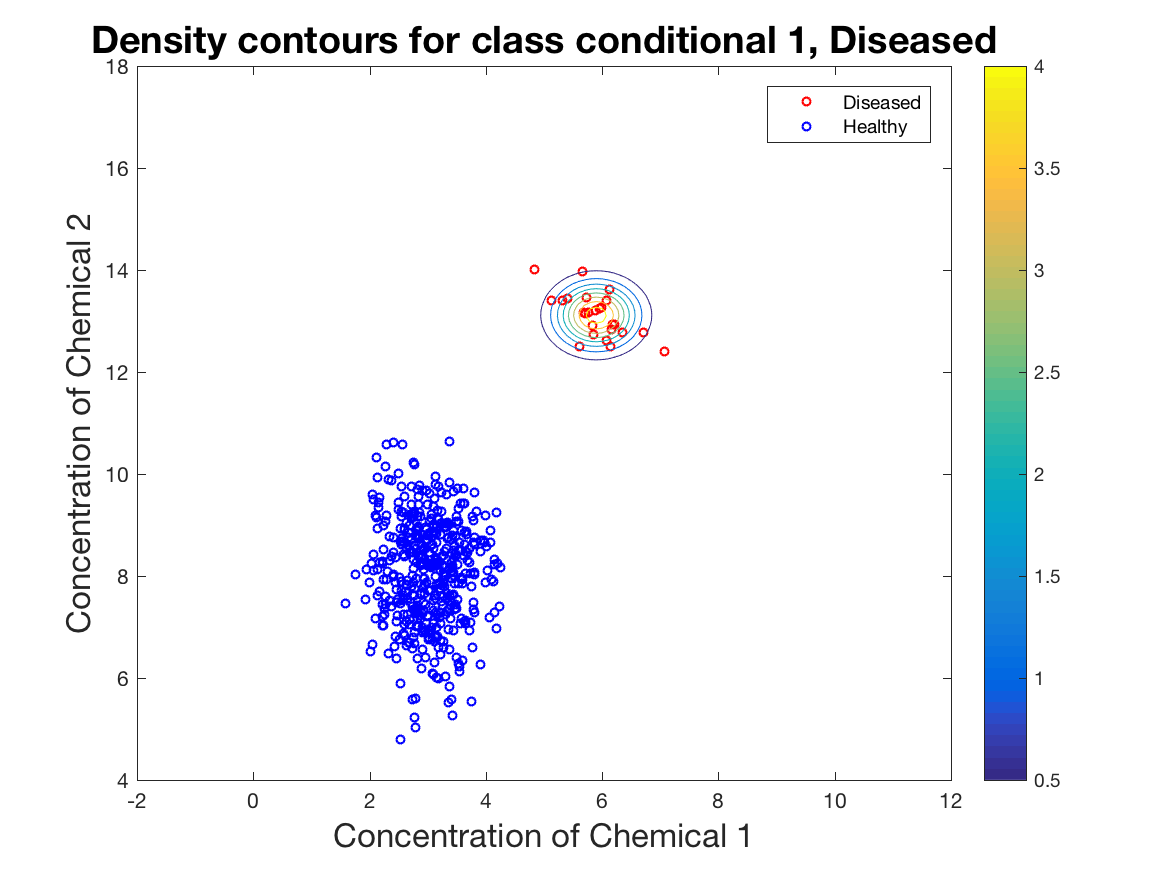
\includegraphics[width=\textwidth]{MLclassCondContoursDiseased.png}
		\caption{ML class conditional 1 density contours}
		\label{fig:cml1}
	\end{subfigure}
	\begin{subfigure}[b]{.40\textwidth}
		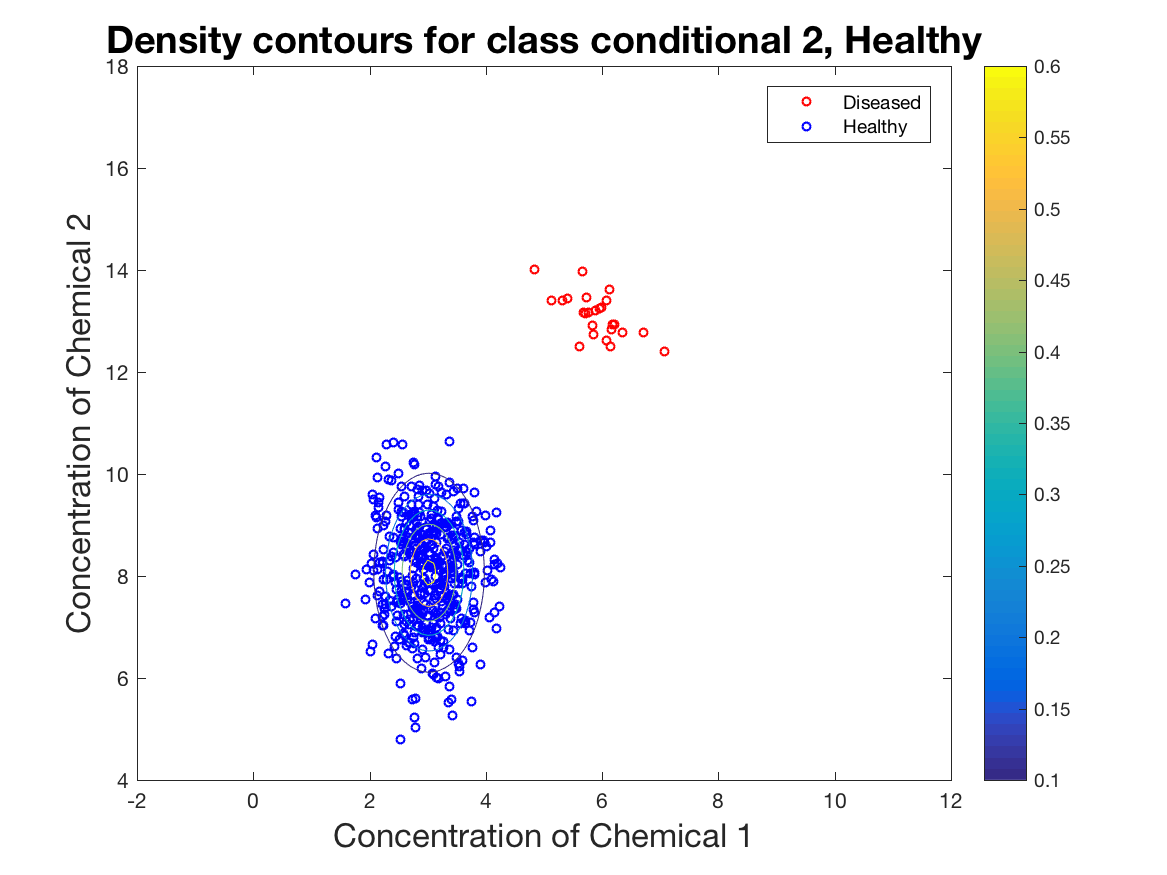
\includegraphics[width=\textwidth]{MLclassCondContoursHealthy.png}
		\caption{ML class conditional 2 density contours}
		\label{fig:cml2}
	\end{subfigure}
	\begin{subfigure}[b]{.40\textwidth}
		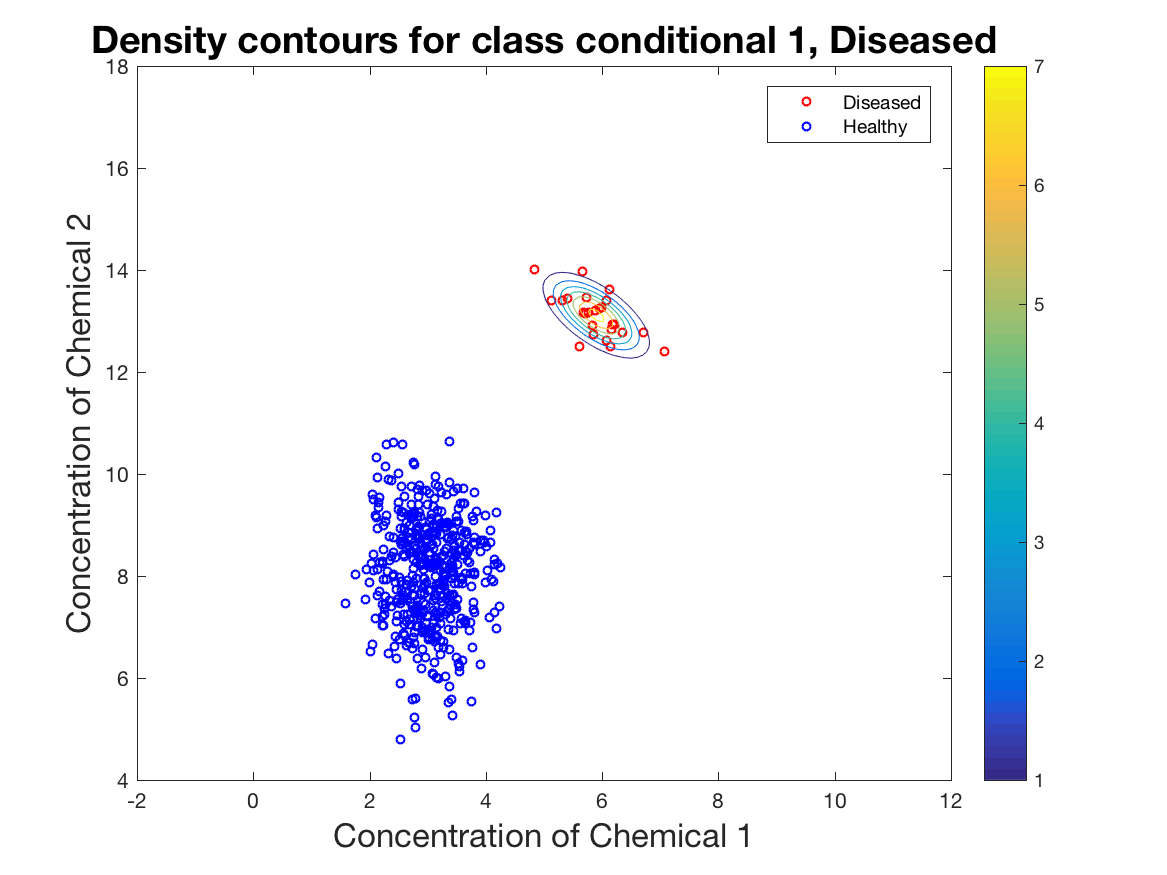
\includegraphics[width=\textwidth]{MLWONclassCondContoursDiseased.png}
		\caption{MLWON class conditional 1 density contours}
		\label{fig:cml3}
	\end{subfigure}
	\begin{subfigure}[b]{.40\textwidth}
		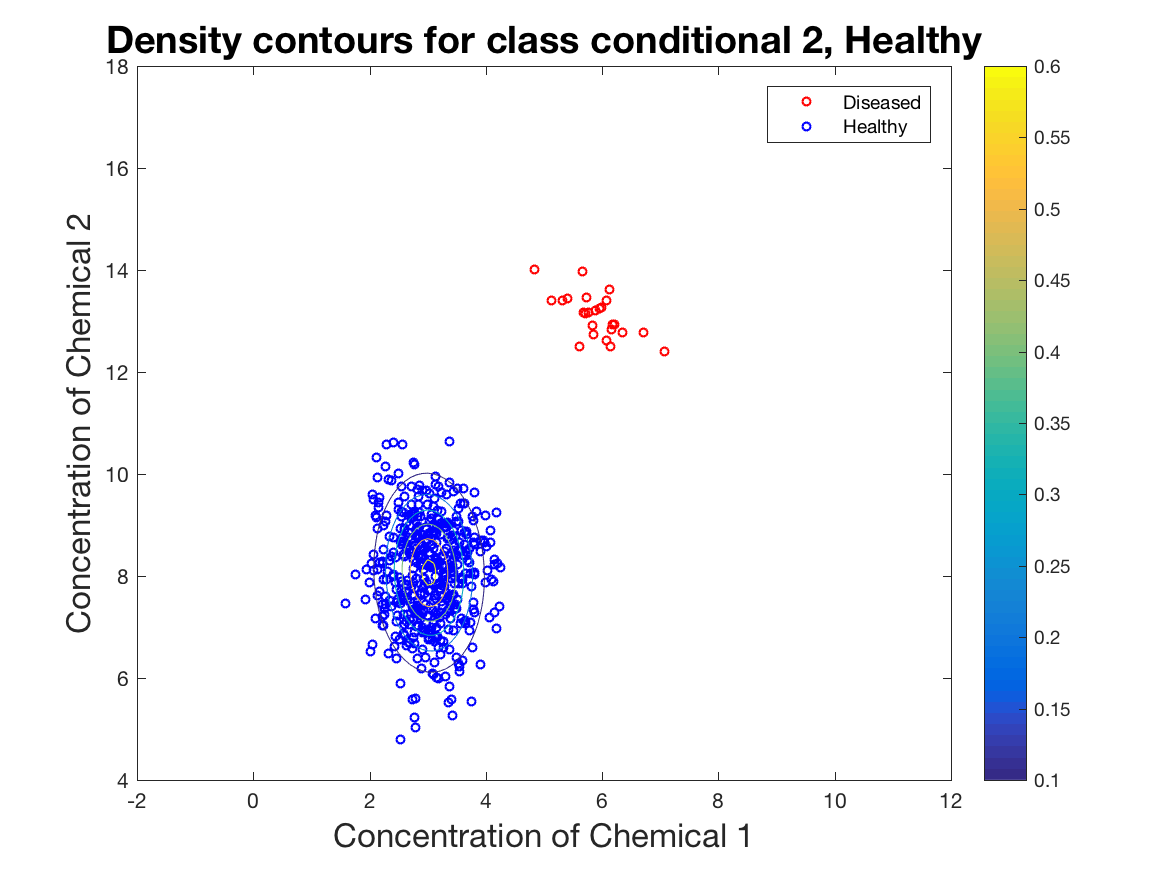
\includegraphics[width=\textwidth]{MLWONclassCondContoursHealthy.png}
		\caption{MLWON class conditional 1 density contours}
		\label{fig:cml4}
	\end{subfigure}
	\caption{Comparison of class conditional density contours for each class and with Naive and without Naive assumption}
	\label{fig:CMLdens}
\end{figure}

The probability contours in Figure \ref{CMLprob} reinforce what we deduced in the density contour plots. This is because they are very much dependent on each other. To generate the probability contours we normalise the maximum likelihood by dividing it with the sum of the ML for each class. Therefore, the probability contour plots are the normalised versions of the maximum likelihood density plots. These are useful as the contours represent actual probabilities rather than some scaled unit.

Interestingly, the probability contours are elliptical (or spherical) around the diseased class for both class 1 and 2. This is again due to the low covariance (or variance) of the diseased data points, which allows class 1 to dominate in terms of probability. This is exacerbated by the imbalanced data set. The healthy patients outnumber the diseased by 19 to 1 (475 vs 25). This means we get more varied values and thus a larger covariance (or variance). This imbalance also has other influences on the prior which is discussed in the following section.

\begin{figure}[h!] 
	\centering
	\begin{subfigure}[b]{.40\textwidth}
		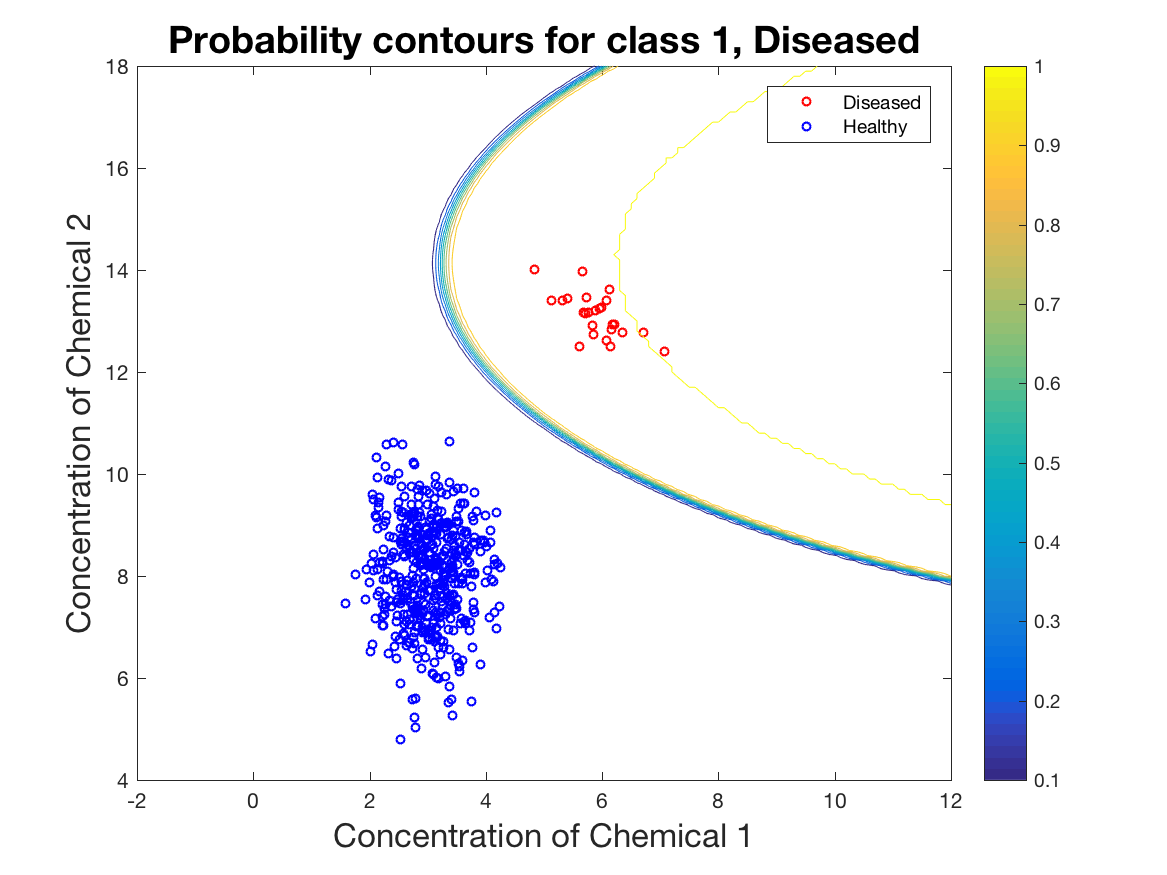
\includegraphics[width=\textwidth]{MLprobContoursDiseased.png}
		\caption{ML probability contours for class 1}
		\label{fig:model0}
	\end{subfigure}
	\begin{subfigure}[b]{0.40\textwidth}
		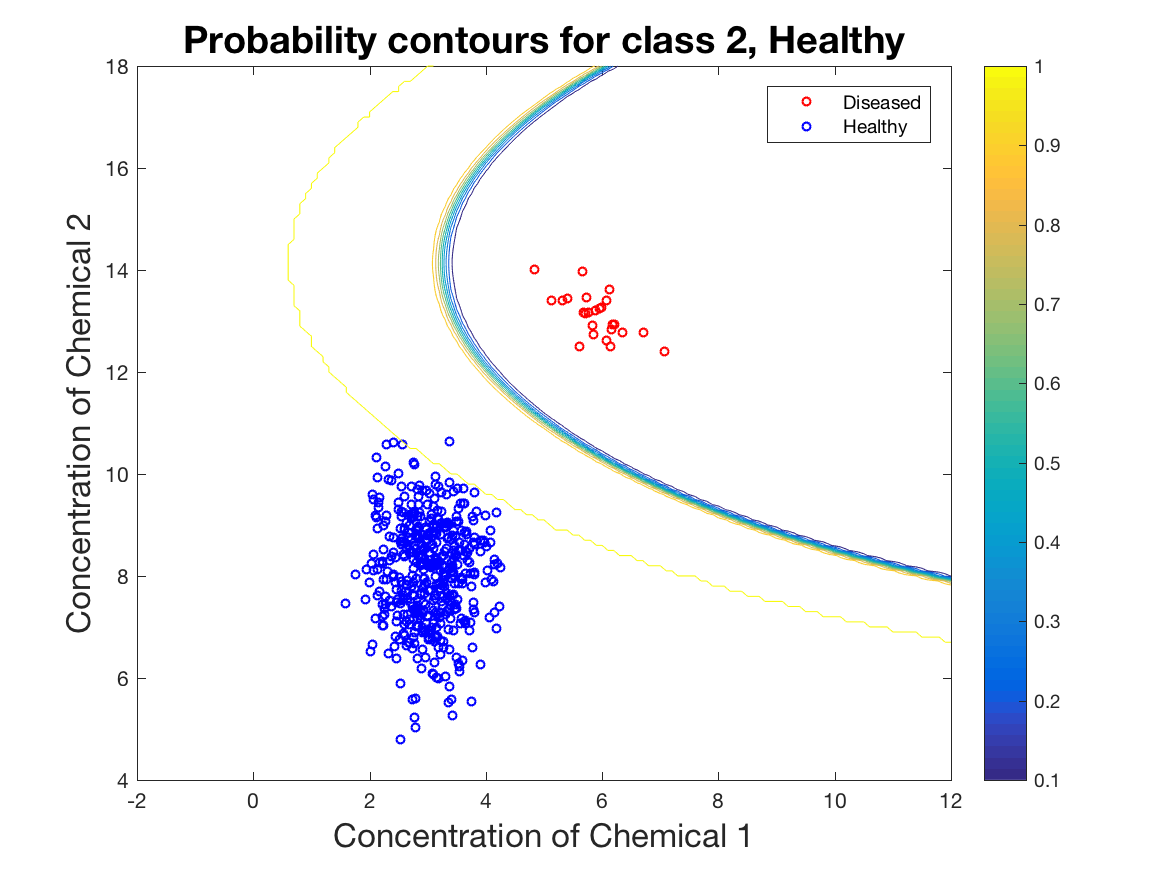
\includegraphics[width=\textwidth]{MLprobContoursHealthy.png}
		\caption{ML probability contours for class 2}
		\label{fig:model1}
	\end{subfigure}
	\begin{subfigure}[b]{.40\textwidth}
		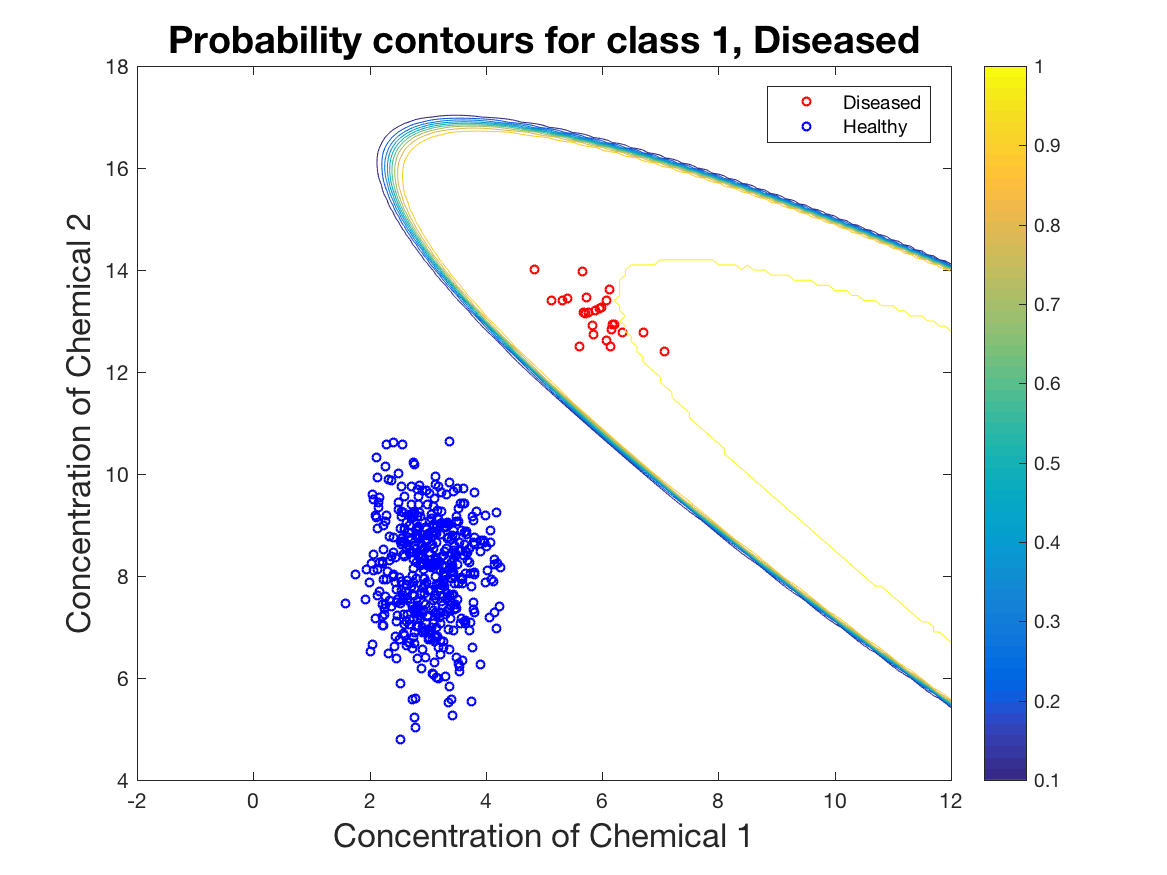
\includegraphics[width=\textwidth]{MLWONprobContoursDiseased.png}
		\caption{MLWON probability contours for class 1}
		\label{fig:model2}
	\end{subfigure}
	\begin{subfigure}[b]{.40\textwidth}
		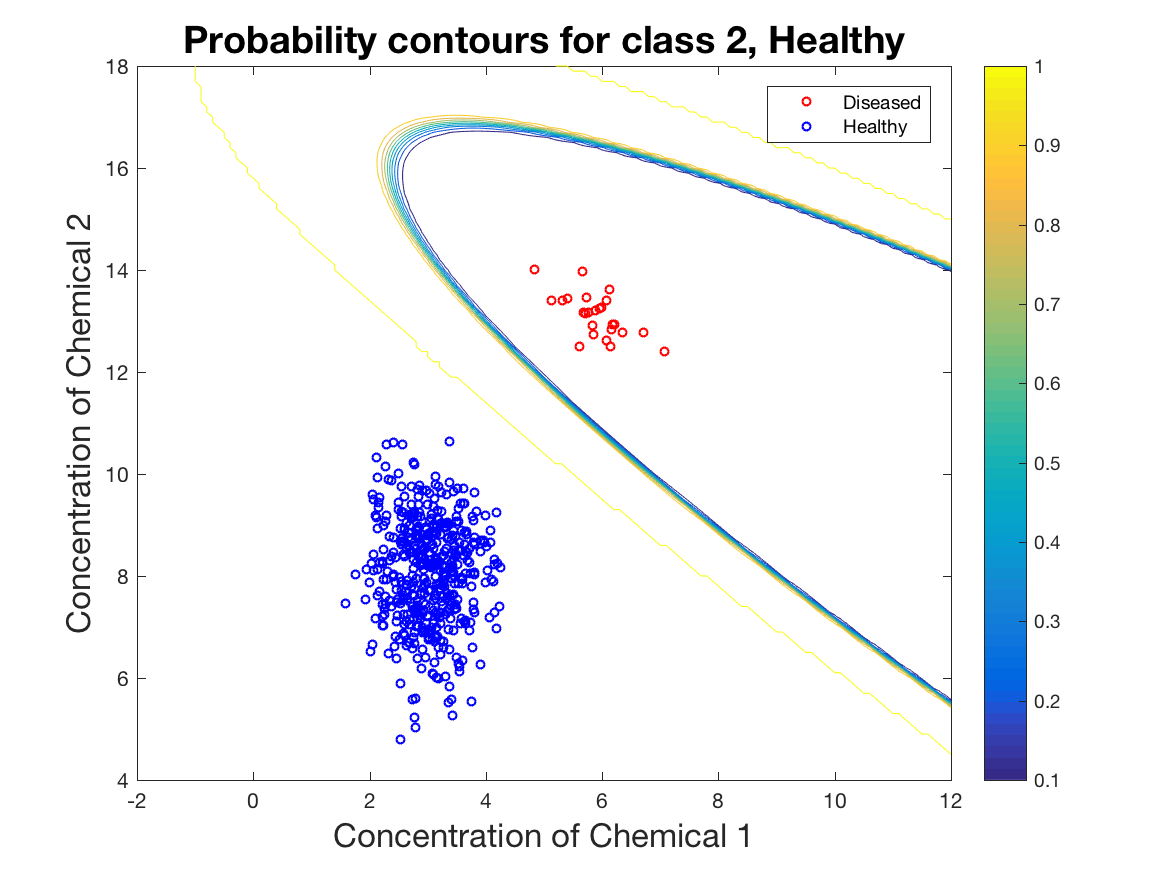
\includegraphics[width=\textwidth]{MLWONprobContoursHealthy.png}
		\caption{MLWON probability contours for class 2}
		\label{fig:model3}
	\end{subfigure}
	\caption{Comparison of probability contours for each class and with Naive and without Naive assumption}
	\label{fig:CMLprob}
\end{figure}

\newpage
\section{Maximum A Posteriori (MAP)}{\label{s1}
	
	\subsection{Introduction}\label{Int}
In Task 1, we are asked to ``train the Bayesian classifier, with maximum likelihood estimate (ML), on the training data with and without the Naive assumption.'' The data set is the one shown in \ref{fig:trainingData}. Once trained we classify 2000 new data points (patients).

To train ML with the Naive assumption first compute the mean and variance of the data for each class and attribute. As it is Naive, we assume the attributes (chemical 1 and 2) are independent. Armed with the mean, variance, and the new data set we use the Gaussian expression to compute the likelihood of each data point as either diseased or healthy. In this case, we are looking at the maximum likelihood and thus, only use class-conditional likelihood to classify. 

To train ML without the Naive assumption is similar to before. We compute the mean as normal but this method requires the covariance not variance of the classes and attributes. This assumes a dependence between the attributes which is useful to look at if there are not many attributes. We then compute the maximum likelihood as normal but accounting for the 3 dimensional matrix due to the covariance.
	
	\subsection{Results}\label{CVcons}
	From Figure \ref{fig:CVT4} and Table \ref{t:ModLoss} it is shown that a polynomial function with order 4 is the best fit. However, in order to determine the "best" order, it must be given a concrete meaning for this task. "Best" is considered to be the minimum mean squared loss, where loss is the difference between predicted and observed labels. Ideally, both cross-validation (CV) and training loss are considered but that is not always the case. So, three cases are defined as the following.
	
	\begin{enumerate}
		\item Only CV loss is considered
		\item Only Train loss is considered
		\item Both CV and Train loss are considered
	\end{enumerate}
	
	\begin{figure}[h]
		\centering
		\includegraphics[width=0.8\linewidth]{images/MAPnewData}
		\caption{Maximum A Posteriori classification of new data}
		\label{fig:MAP}
	\end{figure}
	
	\begin{figure}[h]
		\centering
		\includegraphics[width=0.8\linewidth]{images/MAPWONnewData}
		\caption{Maximum A Posteriori without Naive assumption classification of new data}
		\label{fig:MAPWON}
	\end{figure}
	
	\begin{table}[h]
		\centering
		\caption{Classification Differences between Methods}
		\label{t:ModLoss}
		\begin{tabular}{rrrr}
			\hline
			\textbf{Order} & \textbf{CV Loss} & \textbf{Train Loss} & \textbf{Average Squared Loss} \\ \hline
			0 & 10.83 & 8.07 & 178.61 \\
			1 & 2.71 & 1.54 & 9.03 \\
			2 & 1.57 & 1.01 & 3.33 \\
			3 & 3.99 & 0.98 & 12.35 \\
			4 & 1.64 & 0.93 & 3.30
		\end{tabular}
	\end{table}
	
	Consider item 1, Figure \ref{fig:CVT4} and Table \ref{t:ModLoss} show that a polynomial function with order 2 is the best fit. It is visualised clearly on Figure \ref{fig:CVT4} as the minimum point on the line. Looking at Table \ref{t:ModLoss}, a minimum value of 1.57 also corresponds with order 2.
	
	Consider item 2, Figure \ref{fig:CVT4} and Table \ref{t:ModLoss} show that a polynomial function with order 4 is the best fit. Figure \ref{fig:CVT4} shows a downward trend to the right, indicating that an order of 4 is indeed the best fit. Looking at Table \ref{t:ModLoss}, the minimum value, 3.30, also corresponds with an order of 4.
	
	Consider item 3, Figure \ref{fig:CVT4} and Table \ref{t:ModLoss} show that a polynomial function with order 4 is the best fit. It is difficult to see this via the visualisation of Figure \ref{fig:CVT4}. However, looking at Table \ref{t:ModLoss}, the average squared loss (of CV and Train loss) is lowest when order equals 4. 
	
	Figure \ref{fig:model2} shows how well each of the models fit the data. Interestingly, Figure \ref{fig:model4}, shows an order of 4 provides an accurate model and more realistic future predictions than an order of 2. In comparison, an order of 2 shows that future predictions would increase in time at an increasing rate. This is highly unlikely given the downward trend of the data.
	
	The remaining models in Figure \ref{men400-1} clearly do not model the data well, where orders 1 and 3 show that a time of 0 will be achieved soon. This is not humanly possibly so the models can be discarded. 
	
	\subsection{Conclusion}
	The problem for Task 1 is to find the "best model based on average cross-validation loss." This only considers point 1 from before, therefore, a polynomial function with order 2 best fits the model based on average cross-validation loss.
	
	\begin{figure}[h!] 
		\centering
		\begin{subfigure}[b]{.49\textwidth}
			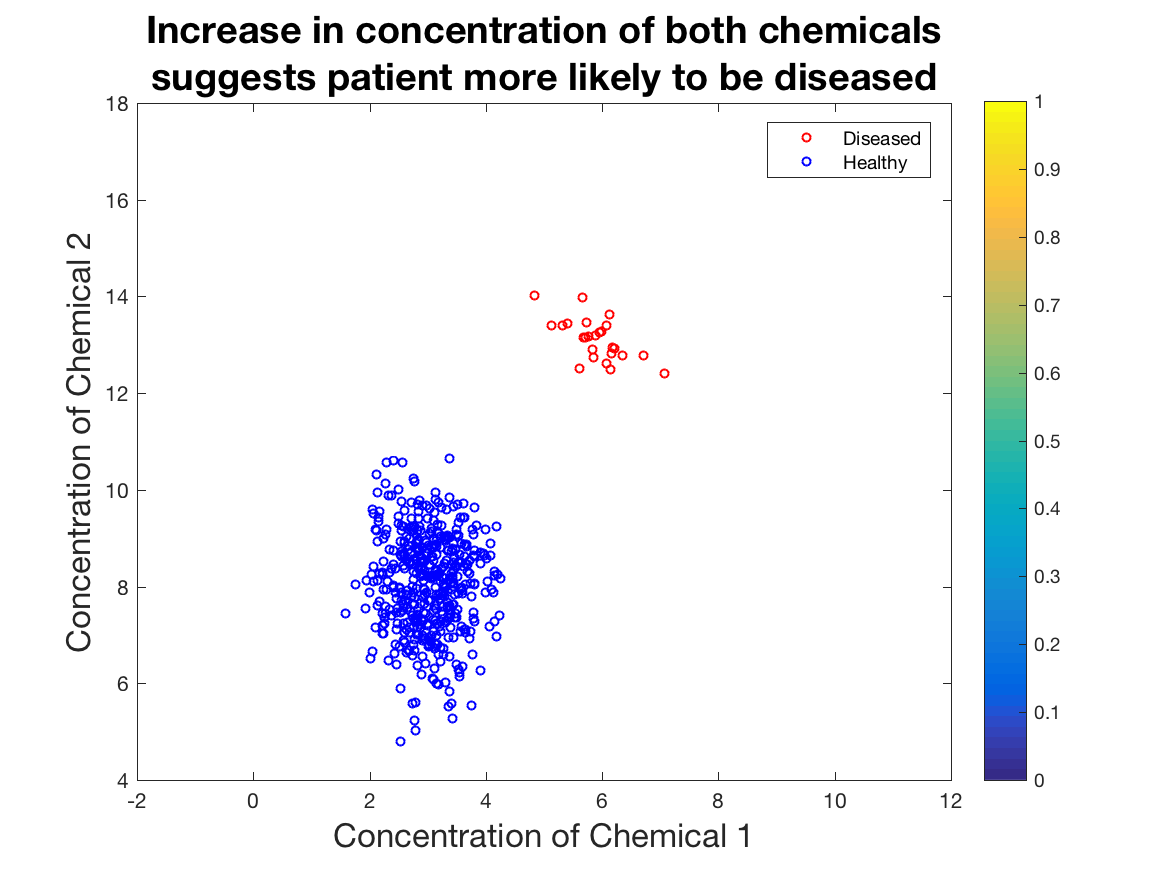
\includegraphics[width=\textwidth]{MAPtrainingData.png}
			\caption{Training data}
			\label{fig:modelNoReg0}
		\end{subfigure}
		\begin{subfigure}[b]{.49\textwidth}
			\includegraphics[width=\textwidth]{MAPnewData.png}
			\caption{Maximum A Posteriori classification of new data}
			\label{fig:modelNoReg1}
		\end{subfigure}
		\begin{subfigure}[b]{.49\textwidth}
			\includegraphics[width=\textwidth]{MAPWONnewData.png}
			\caption{Maximum A Posteriori without Naive assumption classification of new data}
			\label{fig:modelNoReg1}
		\end{subfigure}
		\caption{Comparison of training data and classification of new data by MAP and MAPWON}
		\label{fig:CMAP}
	\end{figure}
	
	\subsection{Further Comments}
	Further investigation found if the data was not standardised, a systematic error is produced in the model for orders greater than or equal 4. Figure \ref{men400-1noSt} illustrates an order of 3 produces no error, but an order of 4 does. Reviewing literature showed this systematic error is common when dealing with high order polynomial function\cite{WhenIsIt}.Therefore, it is good practice to standardise data when the regression model contains polynomial terms.
	
	\begin{figure}[h!] 
		\centering
		\begin{subfigure}[b]{.49\textwidth}
			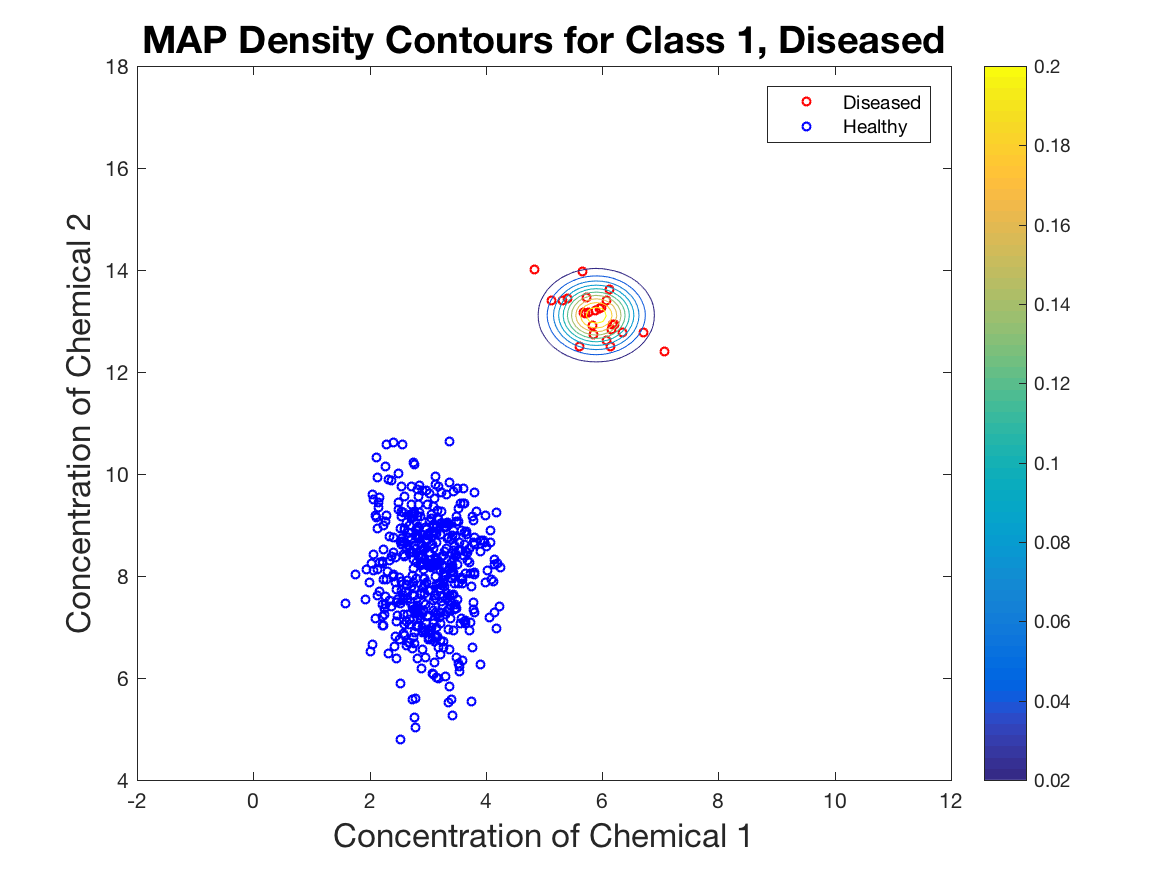
\includegraphics[width=\textwidth]{MAPclassCondContoursDiseased.png}
			\caption{MAP density contours for class 1}
			\label{fig:model0}
		\end{subfigure}
		\begin{subfigure}[b]{.49\textwidth}
			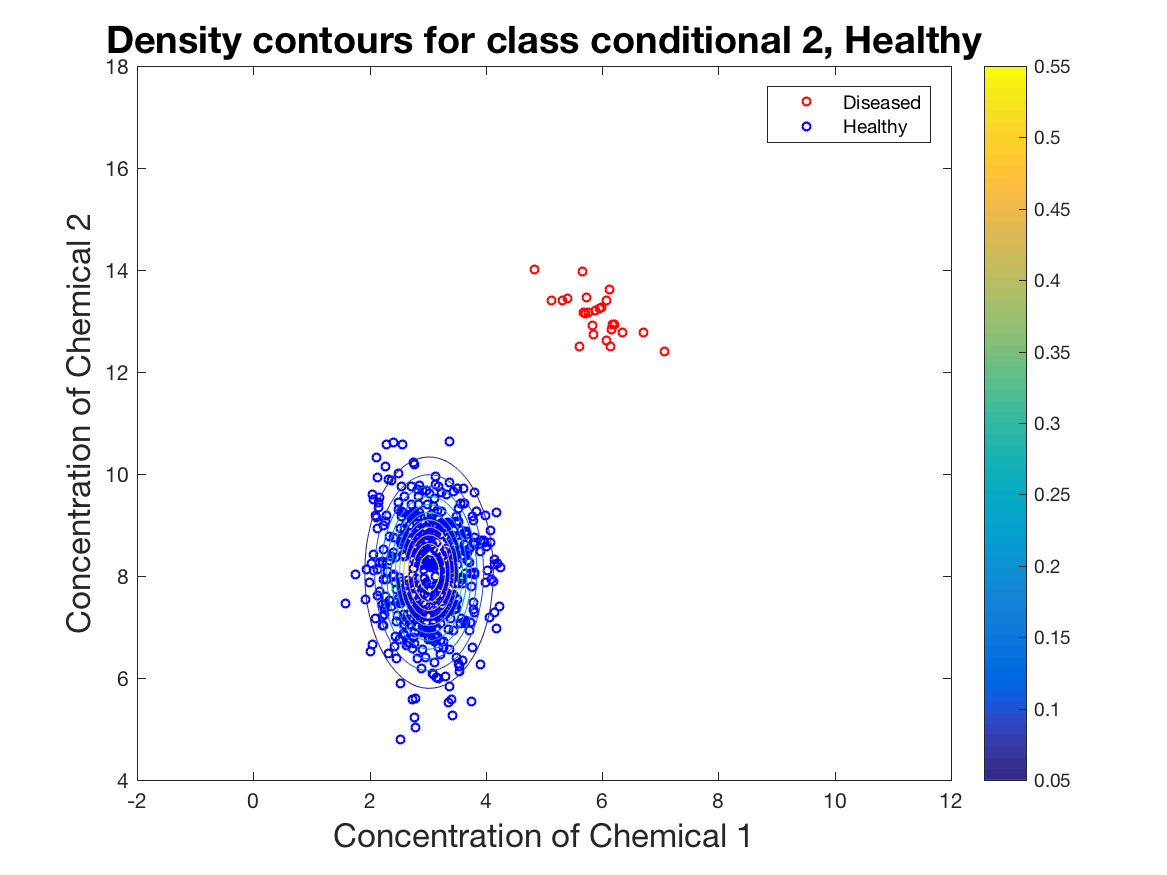
\includegraphics[width=\textwidth]{MAPclassCondContoursHealthy.png}
			\caption{MAP density contours for class 2}
			\label{fig:model1}
		\end{subfigure}
		\begin{subfigure}[b]{.49\textwidth}
			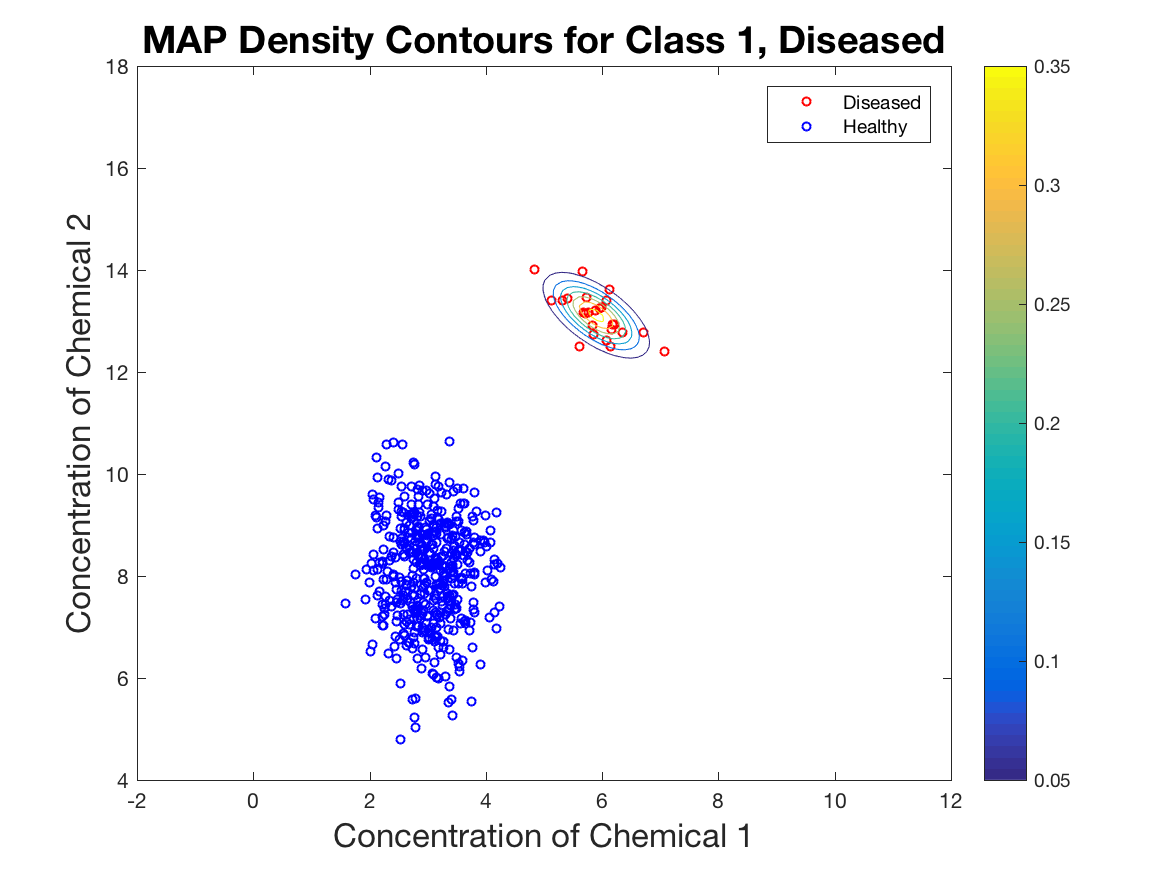
\includegraphics[width=\textwidth]{MAPWONclassCondContoursDiseased.png}
			\caption{MAPWON density contours for class 1}
			\label{fig:model2}
		\end{subfigure}
		\begin{subfigure}[b]{.49\textwidth}
			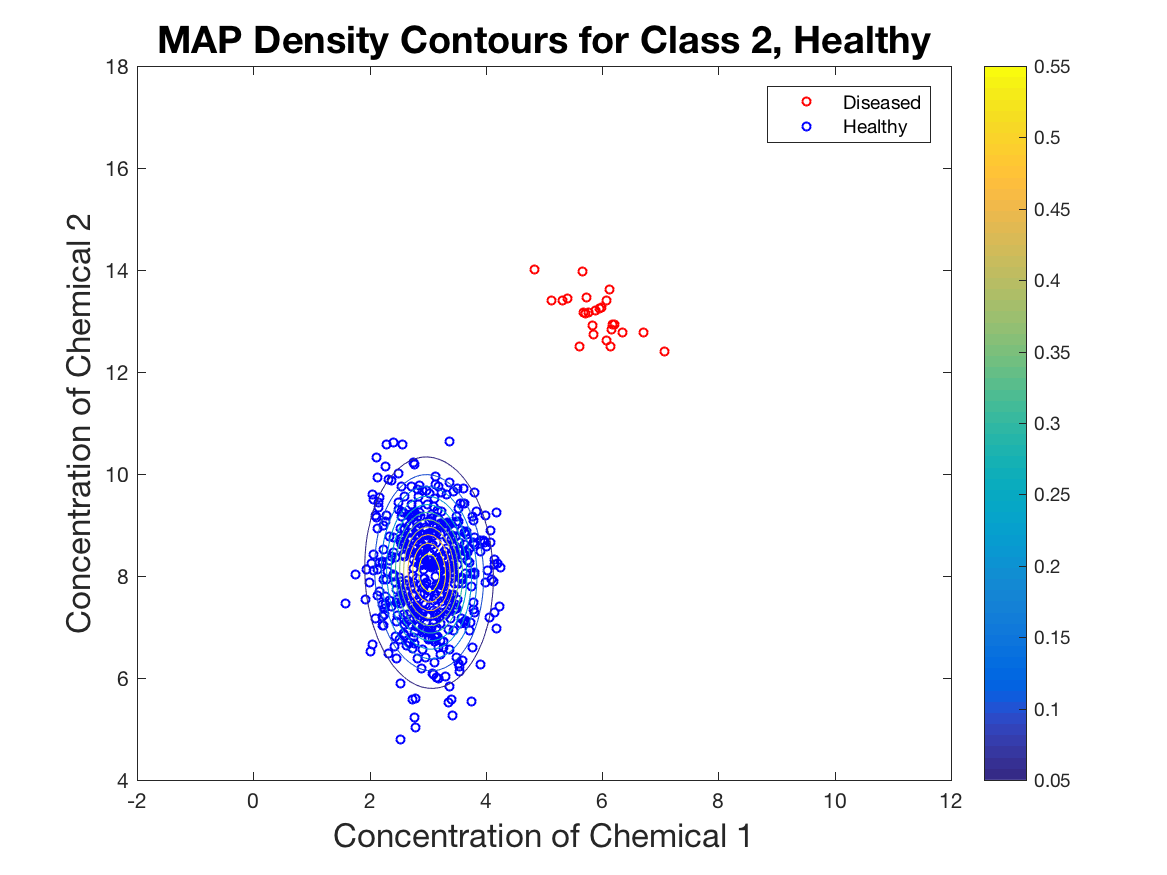
\includegraphics[width=\textwidth]{MAPWONclassCondContoursHealthy.png}
			\caption{MAPWON density contours for class 2}
			\label{fig:model3}
		\end{subfigure}
		\caption{Comparison of density contours for each class and with Naive and without Naive assumption}
		\label{fig:CMAPdens}
	\end{figure}
	
	\begin{figure}[h!] 
		\centering
		\begin{subfigure}[b]{.49\textwidth}
			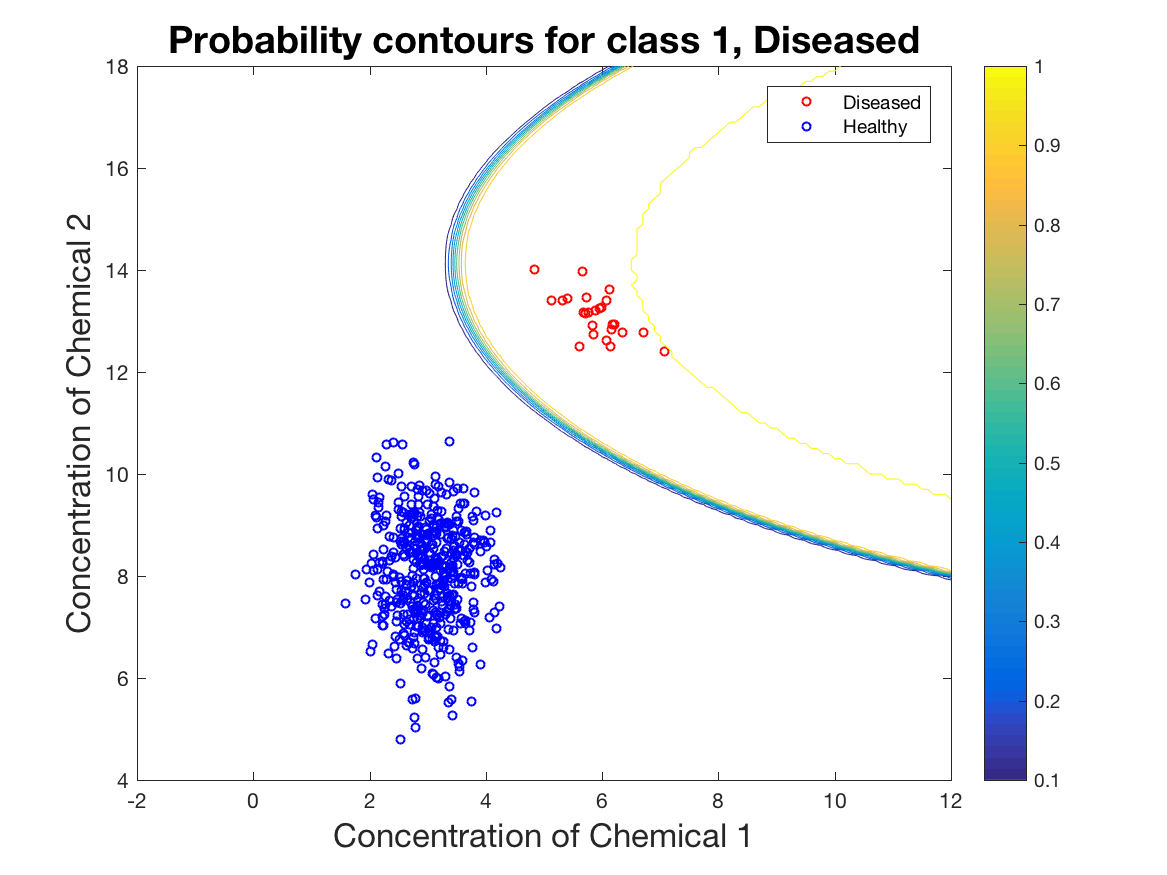
\includegraphics[width=\textwidth]{MAPprobContoursDiseased.png}
			\caption{MAP probability contours for class 1}
			\label{fig:model0}
		\end{subfigure}
		\begin{subfigure}[b]{.49\textwidth}
			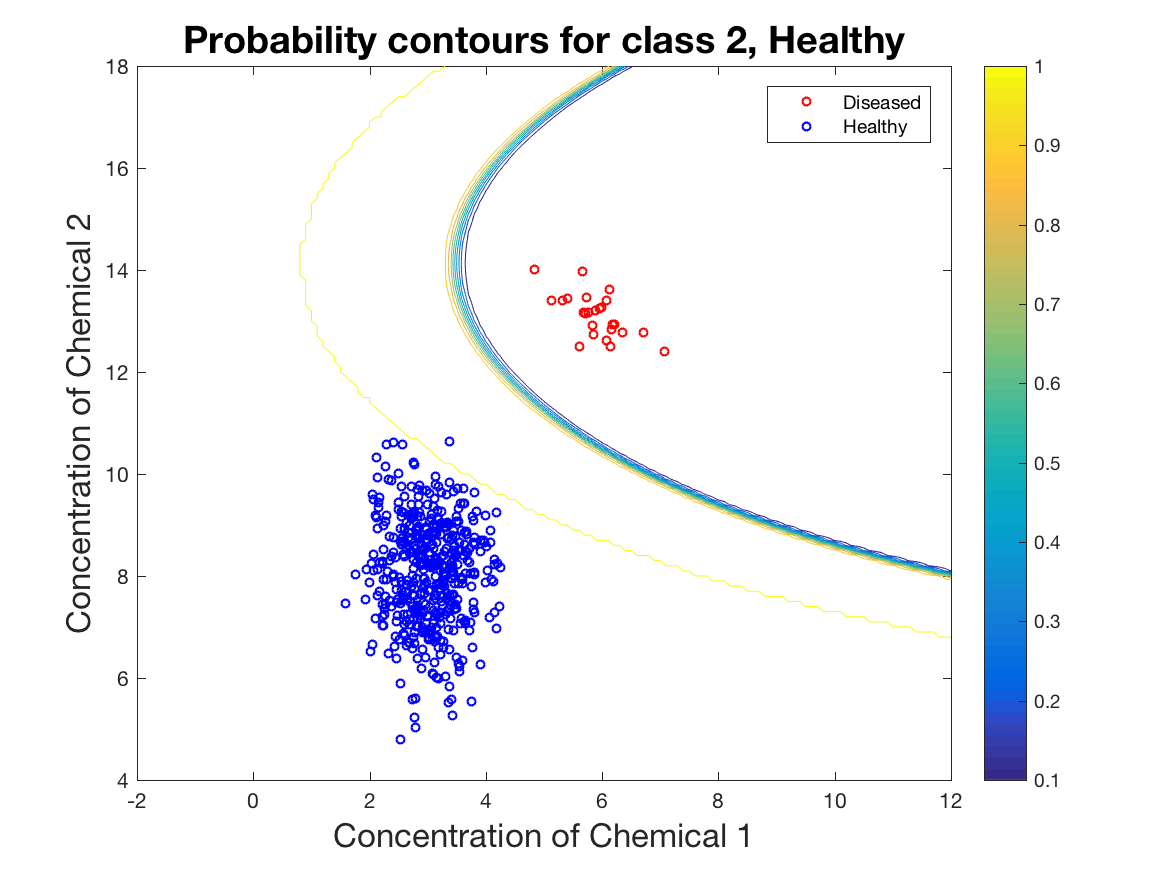
\includegraphics[width=\textwidth]{MAPprobContoursHealthy.png}
			\caption{MAP probability contours for class 2}
			\label{fig:model1}
		\end{subfigure}
		\begin{subfigure}[b]{.49\textwidth}
			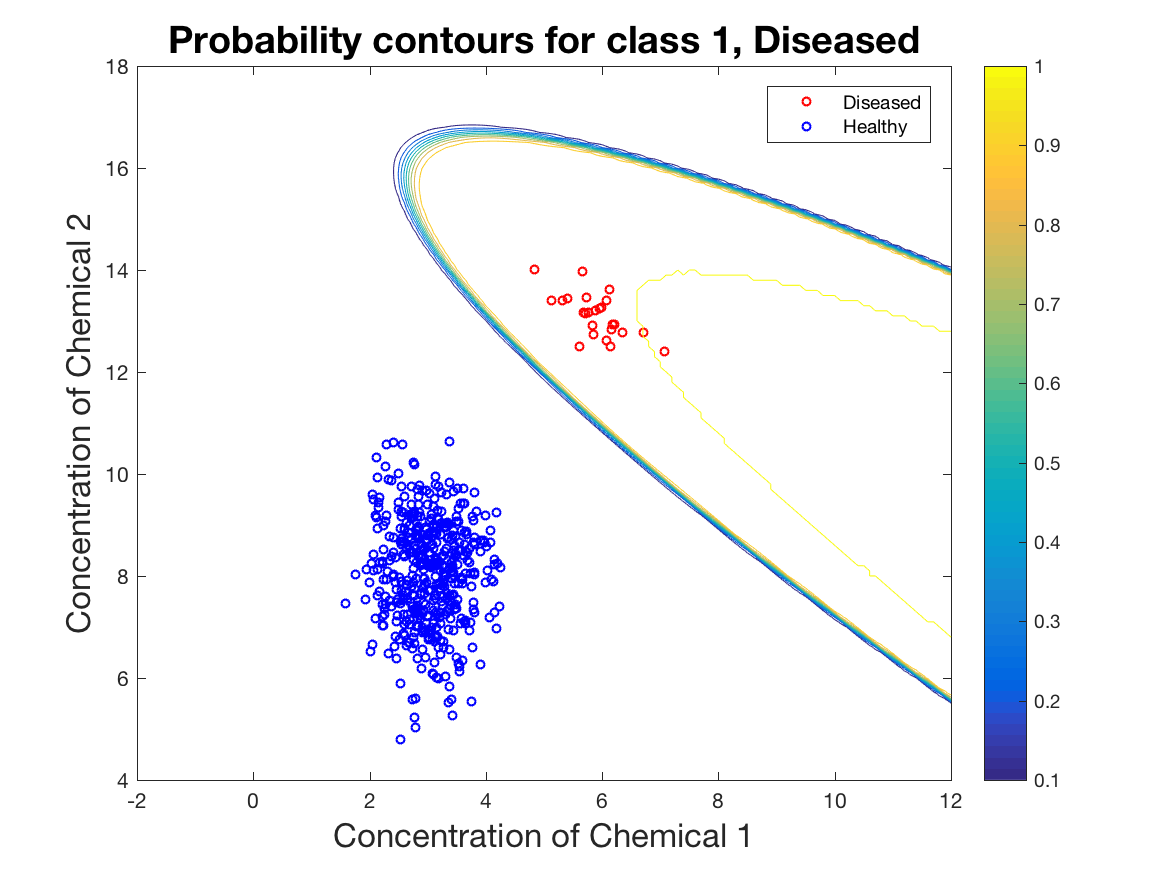
\includegraphics[width=\textwidth]{MAPWONprobContoursDiseased.png}
			\caption{MAPWON probability contours for class 1}
			\label{fig:model2}
		\end{subfigure}
		\begin{subfigure}[b]{.49\textwidth}
			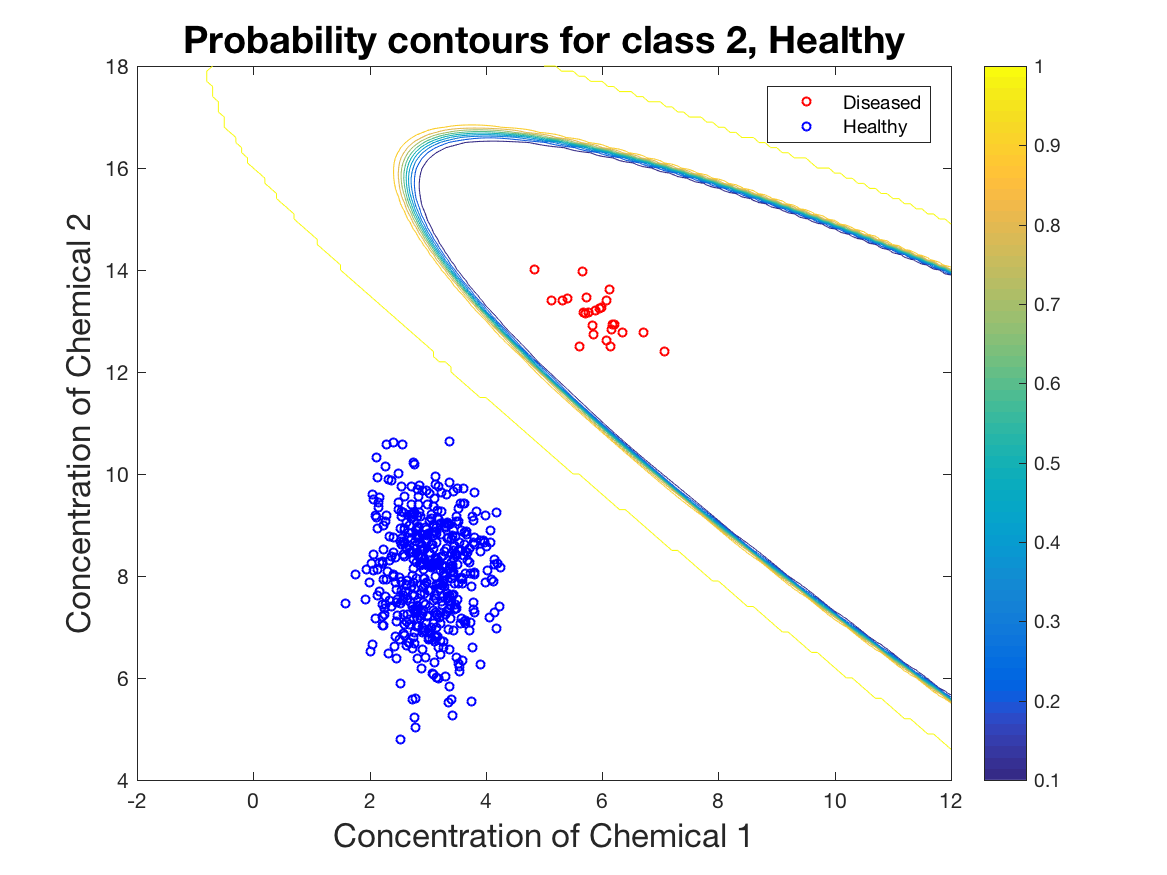
\includegraphics[width=\textwidth]{MAPWONprobContoursHealthy.png}
			\caption{MAPWON probability contours for class 2}
			\label{fig:model3}
		\end{subfigure}
		\caption{Comparison of probability contours for each class and with Naive and without Naive assumption}
		\label{fig:CMAPprob}
	\end{figure}
	
	Another point worth mentioning is the effect of permuting (randomising) the attributes. For this small dataset the permutations caused some instability in the model and different results were obtained as can be seen in Figure \ref{men400CVRandSt}. The results of the permuted data agree with the results from before.
	
\newpage	
\section{Maximum Likelihood vs Maximum A Posteriori  \\ (ML VS MAP)}{\label{s1}
	
	\subsection{Difference of ML and MAP}\label{Int}
	In Task 1, we are asked to analyse the Olympics men's 400m data. We must find the polynomial function of order \textbf{n} which best fits this data, where \textbf{n} is 1 to 4, and use 10-fold cross-validation to choose the "best" value of \textbf{n}. Refer to Appendix A for the Matlab code used for analysis.
	
	\begin{figure}[h!] 
		\centering
		\begin{subfigure}[b]{.49\textwidth}
			\includegraphics[width=\textwidth]{MLnewData.png}
			\caption{Maximum Likelihood classification of new data}
			\label{fig:model0}
		\end{subfigure}
		\begin{subfigure}[b]{.49\textwidth}
			\includegraphics[width=\textwidth]{MLWONnewData.png}
			\caption{Maximum Likelihood WON classification of new data}
			\label{fig:model1}
		\end{subfigure}
		\begin{subfigure}[b]{.49\textwidth}
			\includegraphics[width=\textwidth]{MAPnewData.png}
			\caption{Maximum A Posteriori classification of new data}
			\label{fig:model2}
		\end{subfigure}
		\begin{subfigure}[b]{.49\textwidth}
			\includegraphics[width=\textwidth]{MAPWONnewData.png}
			\caption{Maximum A Posteriori WON classification of new data}
			\label{fig:model3}
		\end{subfigure}
		\caption{Comparison of classification of new data by ML, MLWON, MAP, and MAPWON}
		\label{fig:overallC}
	\end{figure}

\begin{table}[h]
	\centering
	\caption{Classification Differences between Methods}
	\label{t:classNumber}
	\begin{tabular}{lrr}
		\hline
		\textbf{Method} & \textbf{Classified as Diseased} & \textbf{Classified as Healthy}\\ \hline
		ML & 764 & 1236 \\
		MLWON& 681 & 1319 \\
		MAP & 826 & 1174  \\
		MAPWON & 749 & 1254 \\
	\end{tabular}
\end{table}
	
	To compute the average cross validation loss, data (attributes and labels) are separated into 10 partitions (i.e. 10-fold), where 1 partition is reserved for testing the model. The 9 remaining partitions are used to learn the model with parameters, $w_{n}$. This models can use the attributes of the test partition to predict the labels, in this case the time ran for the men's 400m. The predicted values can then be compared to the actual values (labels)  from the test partition. The cross validation (CV) loss is calculated by taking the mean squared difference ($msd$) of these two values. This is then repeated 9 more times by rotating the test partition through. The average of these 10 $msd$ values is calculated and then plotted against the order to find the minimum value.
	
		\subsection{Affects of Difference on this Data}\label{Int}
	In Task 1, we are asked to analyse the Olympics men's 400m data. We must find the polynomial function of order \textbf{n} which best fits this data, where \textbf{n} is 1 to 4, and use 10-fold cross-validation to choose the "best" value of \textbf{n}. Refer to Appendix A for the Matlab code used for analysis.
	
	To compute the average cross validation loss, data (attributes and labels) are separated into 10 partitions (i.e. 10-fold), where 1 partition is reserved for testing the model. The 9 remaining partitions are used to learn the model with parameters, $w_{n}$. This models can use the attributes of the test partition to predict the labels, in this case the time ran for the men's 400m. The predicted values can then be compared to the actual values (labels)  from the test partition. The cross validation (CV) loss is calculated by taking the mean squared difference ($msd$) of these two values. This is then repeated 9 more times by rotating the test partition through. The average of these 10 $msd$ values is calculated and then plotted against the order to find the minimum value.
	
	Insert Table showing difference!!!
